% =====================================================================
%  第 2.2–2.3 节  例子与图示；Morse 收缩（原书 p.5–9）
% =====================================================================
\subsection{例子与图示}\label{sec:2.2}

\begin{takeaway}
\begin{itemize}
  \item \textbf{物理图像}：在 $T^*X$ 上取 $\epsilon\to0$，全纯圆盘投影到 $X$ 后收缩为梯度流树；复合映射就是这类树的计数。图~\ref{fig:1}--\ref{fig:4} 依次画出无链、单链、多链三种情形。
  \item \textbf{数学工具}：带双指标 $(a,b)$ 的梯度轨道、Morse 树模空间、模空间的维数与平衡条件 $\dim\mathcal M=0$、$\Ainf$ 关系式在 $n=2$ 时的展开。
  \item \textbf{主要结论}：文中各例都是第~\ref{sec:2.1} 节复合映射 \eqref{eq:4} 的特例；例~\ref{ex:3} 表明，$\Ainf$ 关系式的几何含义是一维模空间的带符号边界计数相消为零。
\end{itemize}
\end{takeaway}

上面的定义看起来略嫌繁重，但背后的想法其实直观，可用几个简单例子说明。

\begin{thmenv}{例}{1}\label{ex:1}
复合映射
\[
  m\colon\Mor(F_1,F_2)\otimes\Mor(F_2,F_3)\to\Mor(F_1,F_3)
\]
（不涉及奇异链）由计数如下形状、由梯度轨道拼成的树给出：
\begin{figure}[htbp]
  \centering
  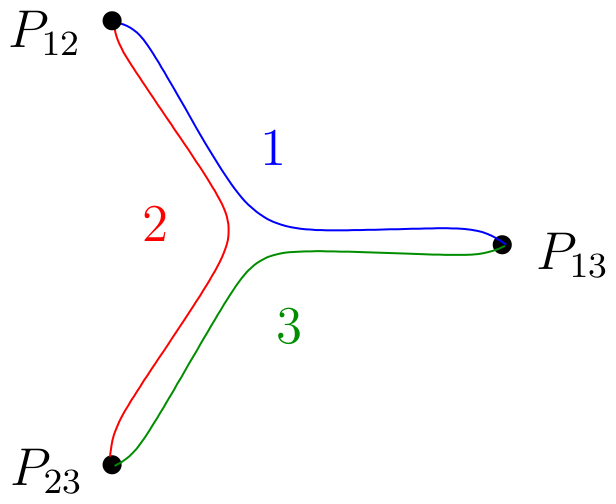
\includegraphics[width=0.35\linewidth]{fig01.png}
  \caption{Morse 树（原书 p.5）}
  \label{fig:1}
\end{figure}
\end{thmenv}

% [Tutor Note: 图 1 中边上的数字 1、2、3 是三个对象的标号（对应图 2 的 $L_1,L_2,L_3$ 即圆盘的三段边界弧），不是边的编号。每条边另带双指标 $(a,b)$ 与方向：$P_{12}$、$P_{23}$ 是叶，$P_{13}$ 是根，方向由叶指向根；方向读反，复合的输入与输出就对调。]

下面这张更细致的图解释这棵树的来源。它来自 $T^*X$ 中 Lagrange 子流形（形如 $L_a=\mathrm{graph}(\epsilon\,\mathrm{d}F_a)$）的 Fukaya 范畴，该范畴的复合映射由全纯圆盘的计数给出：

\begin{figure}[htbp]
  \centering
  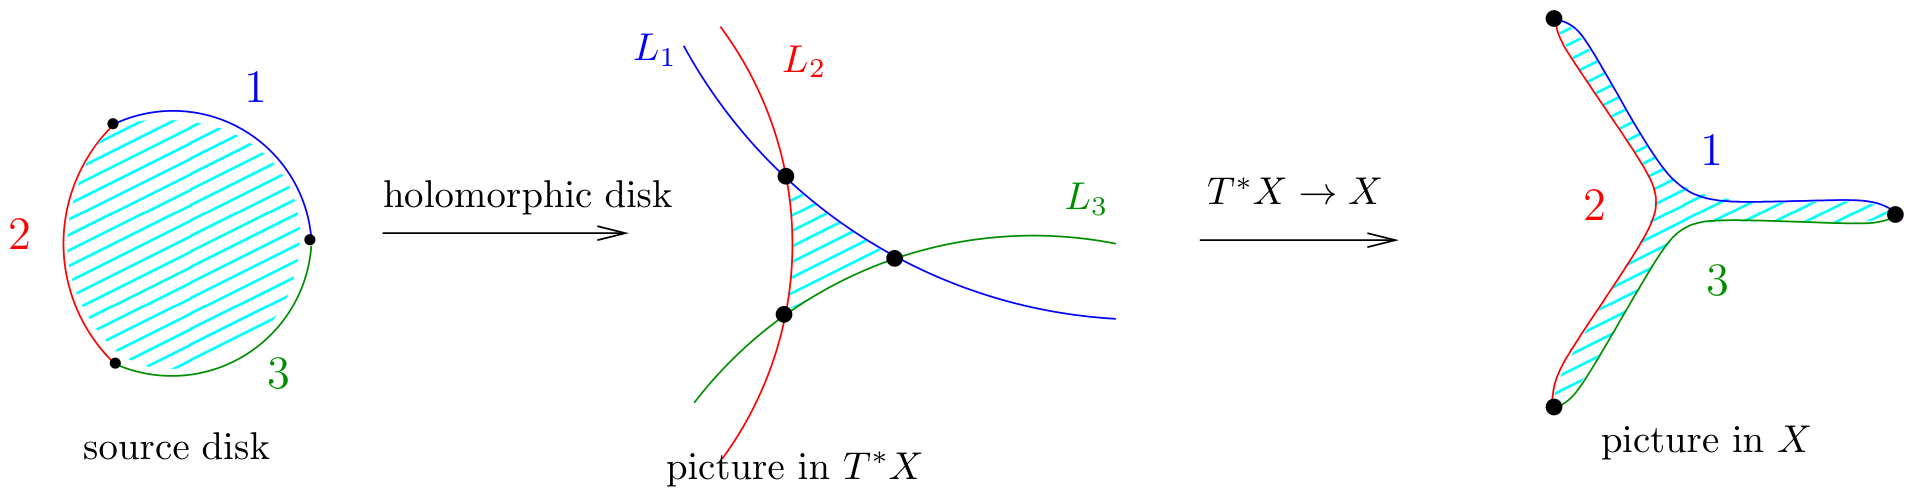
\includegraphics[width=0.76\linewidth]{fig02.png}
  \caption{$X$ 中的 Morse 树：$T^*X$ 中全纯圆盘在 $\epsilon\to0$ 极限下的投影（原书 p.6）}
  \label{fig:2}
\end{figure}

% [Tutor Note: 图 2 中间那幅画在 $T^*X$ 里：$L_a=\mathrm{graph}(\epsilon\,\mathrm{d}F_a)$ 是恰当 Lagrange 子流形，投影 $T^*X\to X$ 把它压到 $X$ 上。$\epsilon\to0$ 时全纯圆盘的面积趋于零，圆盘的极限是梯度流树；这里的“全纯”一律指伪全纯（见第 1 节脚注 1）。紧性论证原文未写，可参看 \cite{fukayaoh}。]

把这张图稍作修改，就得到复合映射
\[
  m\colon\Mor(F_1,F_2)\otimes\Mor(F_2,F_2)\otimes\Mor(F_2,F_3)\to\Mor(F_1,F_3)
\]
的图景；其中用到 $X$ 上（相应地，$T^*X$ 中某个 Lagrange 子流形上）的一条奇异链 $Z\in\Mor(F_2,F_2)$：

\begin{figure}[htbp]
  \centering
  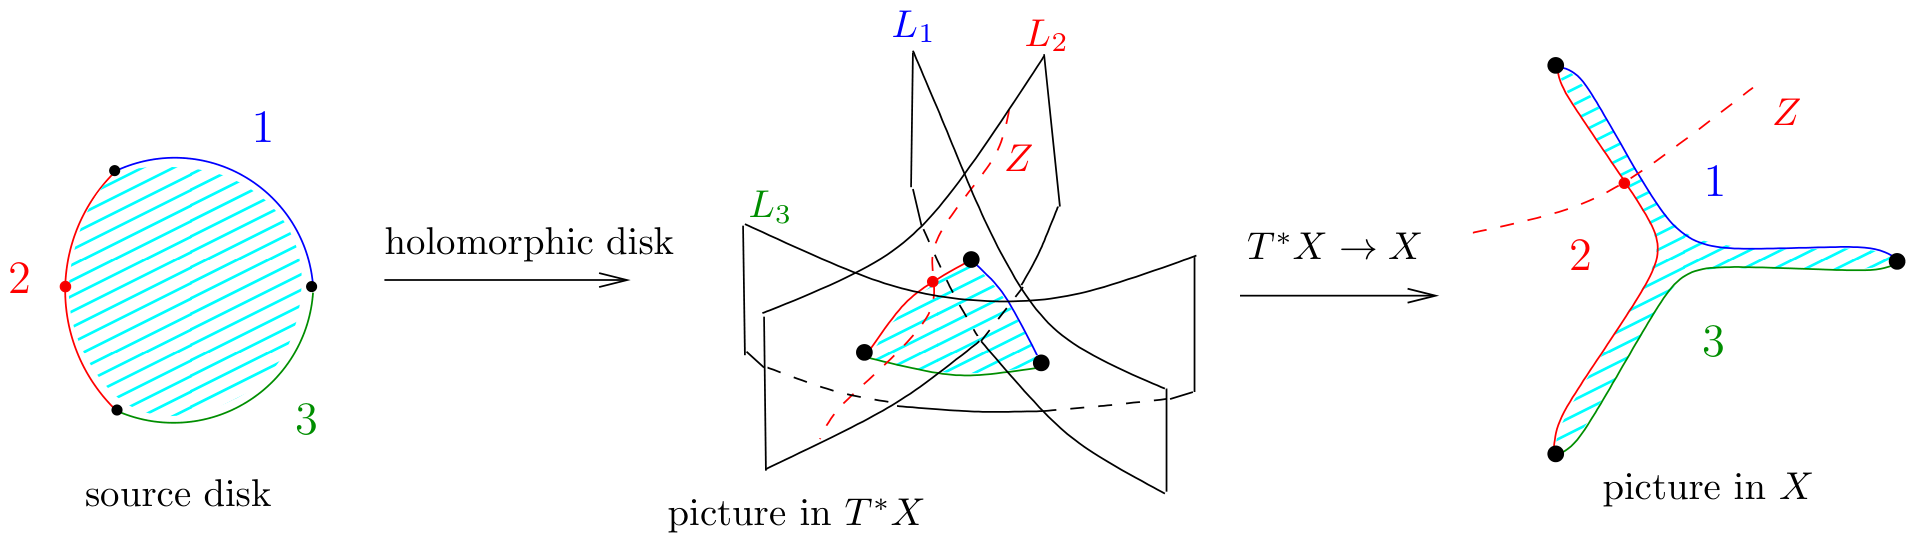
\includegraphics[width=0.76\linewidth]{fig03.png}
  \caption{全纯圆盘与 Morse 树同一条链相交（原书 p.6）}
  \label{fig:3}
\end{figure}

\begin{thmenv}{例}{2}\label{ex:2}
复合映射
\[
  m\colon\Mor(F_1,F_1)^{\otimes k}\otimes\Mor(F_1,F_2)\otimes\Mor(F_2,F_2)^{\otimes l}\to\Mor(F_1,F_2)
\]
由计数 $F_1-F_2$ 的、与给定一族链（图中虚线）相交的梯度轨道给出：
\begin{figure}[htbp]
  \centering
  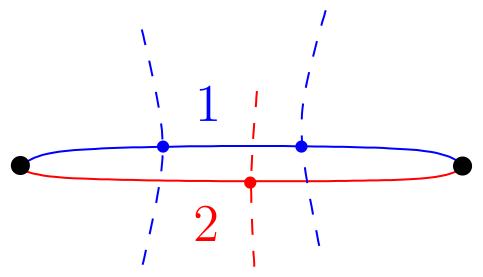
\includegraphics[width=0.20\linewidth]{fig04.png}
  \caption{经过一族链的梯度轨道（原书 p.6）}
  \label{fig:4}
\end{figure}
\end{thmenv}

相应梯度轨道模空间的维数为
\[
  \dim\mathcal M
  =\operatorname{ind}(P)-\operatorname{ind}(P')-1
  -\sum_{\alpha=1}^{k}\bigl(\operatorname{codim}(Z_{\alpha,1})-1\bigr)
  -\sum_{\beta=1}^{l}\bigl(\operatorname{codim}(Z_{\beta,2})-1\bigr).
\]
为使该态射非零，临界点的指标与链的维数须满足平衡条件，即 $\dim\mathcal M=0$。

% [Tutor Note: 维数公式逐项对账：$\operatorname{ind}$ 是 $F_1-F_2$ 的 Morse 指标；$P\to P'$ 的轨道模空间维数为 $\operatorname{ind}(P)-\operatorname{ind}(P')$，再减 1 是去掉梯度流的 $\mathbb R$-平移。每个 2 价顶点是一条边与链 $Z$ 的交点：链的余维数为 $c$ 时只贡献 $c-1$ 个条件，因为交点沿 1 维的边可自动滑动。另注意 (1) 按余指标分次，此处用指标，二者只差常数 $\dim X$，差值不变。]

\begin{thmenv}[$A_\infty$ 关系式的一个例子]{例}{3}\label{ex:3}
取 $X$ 为二维球面，$F_{1,2}$ 为两个函数，使 $F_1-F_2$ 是心形球面的高度函数。设 $P,Q$ 为 $F_1-F_2$ 的两个指标为 2 的临界点，$R$ 为指标为 1 的临界点，$S$ 为指标为 0 的临界点，$Z$ 为一条嵌入区间，如下图。

\begin{figure}[htbp]
  \centering
  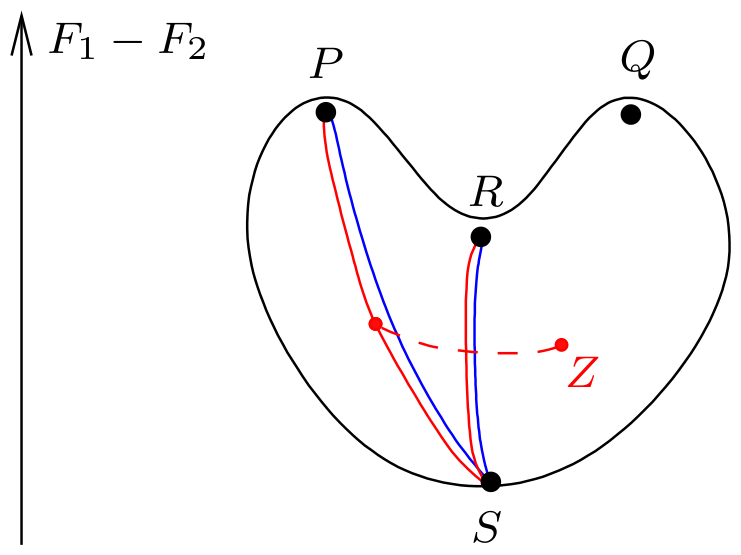
\includegraphics[width=0.30\linewidth]{fig05.png}
  \caption{式~\eqref{eq:8} 的前两项：经过一条链及其边界的梯度轨道（原书 p.7）}
  \label{fig:5}
\end{figure}

有关系式
\begin{equation}\tag{8}\label{eq:8}
  m\bigl(\underbrace{\mathrm{d}_{\mathrm{Morse}}[P]}_{[R]},Z\bigr)
  +m([P],\partial Z)
  +\mathrm{d}_{\mathrm{Morse}}m([P],Z)=0.
\end{equation}
前两项各给出 $S$，且符号相反；第三项为零（因为当 $\widetilde P=S$ 时，模空间 $\mathcal M(P,Z,\widetilde P)$ 是一维的；当 $\widetilde P$ 为其它临界点时，该模空间为空）。这正是 $\Ainf$ 关系式 \eqref{eq:7} 在输入态射 $x_1=[P]$、$x_2=Z$ 下的形式。
\end{thmenv}

% [Tutor Note: 把 (7) 按 $n=2$ 展开：$r=0,s=1$ 给出 $m(\mathrm{d}x_1,x_2)$，$r=1,s=1$ 给出 $m(x_1,\mathrm{d}x_2)$，$r=0,s=2$ 给出 $\mathrm{d}m(x_1,x_2)$，正是 (8) 的三项。注意 $x_2=Z$ 是链，其微分是边界算子，故第二项写作 $m([P],\partial Z)$ 而非 $m([P],\mathrm{d}Z)$；$x_1=[P]$ 是 Morse 链，$\mathrm{d}_{\mathrm{Morse}}[P]=[R]$ 即式 (8) 中的下花括号。]

\subsection{Morse 收缩}\label{sec:2.3}

\begin{takeaway}
\begin{itemize}
  \item \textbf{物理图像}：Morse 收缩把 de Rham 复形压到 Morse 链复形上。$i$ 把临界点打成不稳定流形上的 delta 形式，$p$ 沿稳定流形积分、读回系数，$K$ 沿梯度流积分，给出连接二者的链同伦。
  \item \textbf{数学工具}：$X\times X$ 上的积分核与分布核、奇异支集、正规化数据、光滑化算子 $R_\epsilon$、形变收缩。
  \item \textbf{主要结论}：$(i,p,K)$ 满足 $\mathrm{d}K+K\mathrm{d}=ip-\mathrm{id}$；$K$ 的核是 $\widetilde Y=\cup_{t>0}Y_t$，其边界给出 $Y_{+\infty}-\mathrm{Diag}$；把 $i$、$K$ 光滑化后得到形变收缩 $(i^\epsilon,p,K^\epsilon)$，它是后文证明的关键构件。
\end{itemize}
\end{takeaway}

下一个例子要先回忆 \cite[第 6.5 节]{kontsevichsoibelman} 中的 Morse 收缩构造：它把 de Rham 复形收缩到 Morse 复形。这一构造也是后文几节的关键构件。

设 $F$ 是 $X$ 上的 Morse--Smale 函数，$v$ 是相应的梯度向量场。考虑表达式
\begin{equation}\tag{9}\label{eq:9}
  U(t,\mathrm{d}t)=e^{-t\mathcal L_v}\bigl(1-\mathrm{d}t\,\iota_v\bigr).
\end{equation}
这是 $(0,+\infty)$ 上的非齐次微分形式，取值是作用在 $X$ 的微分形式上的线性算子。\footnote{算子 (9) 是 Morse 拓扑量子力学的演化算子，可理解为度量区间模空间上的一个微分形式，见 \cite{witten,frenkel} 与下文第~\ref{sec:4.1} 节。}下文 $e^{-t\mathcal L_v}$ 一律指沿 $v$ 的流按时间 $-t$ 作拉回。

% [Tutor Note: (9) 中 $\mathcal L_v$ 是李导数，$\iota_v$ 是内乘（interior product）。$U$ 的 0 次部分是拉回 $e^{-t\mathcal L_v}$，1 次部分是 $-\mathrm{d}t\,e^{-t\mathcal L_v}\iota_v$，故 (12) 的负号来自这里；$\int_0^\infty U(t,\mathrm{d}t)$ 只取 $\mathrm{d}t$ 分量，即在 $(0,+\infty)$ 上积一个 1 次形式。把 $\iota_v$ 从 $e^{-t\mathcal L_v}$ 右边挪到左边不变号，因为 $v$ 在自身的流下不变：$e^{-t\mathcal L_v}\iota_v=\iota_v e^{-t\mathcal L_v}$。]

\textbf{未正规化的 Morse 收缩。}\quad 考虑如下三个映射。

\begin{itemize}
  \item 嵌入映射 $i\colon \mathrm{MC}^j(F,\mathbb R)\to\Omega^j_{\mathrm{distr}}(X)$，即把实系数 Morse 复形映入分布形式。它把 $F$ 的余指标为 $j$ 的临界点 $P$ 映为 $P$ 的不稳定流形上的 delta 形式（又称 Lefschetz thimble，莱夫希茨顶针）：
  \begin{equation}\tag{10}\label{eq:10}
    i\colon[P]\mapsto\delta_{\mathrm{Unstab}P}.
  \end{equation}
  \item 投影 $p\colon\Omega^j_{\mathrm{distr}}(X)\to \mathrm{MC}^j(F,\mathbb R)$ 由下式定义：
  \begin{equation}\tag{11}\label{eq:11}
    p\colon\omega\mapsto\sum_{P\in\mathrm{Crit}(F)}
    \Bigl(\int_{\mathrm{Stab}_P}\omega\Bigr)\cdot[P],
  \end{equation}
  其中 $\mathrm{Stab}_P\subset X$ 是 $P$ 的稳定流形。线性算子 $p$ 稠密定义，并满足 $p\circ i=\mathrm{id}_{MC(F)}$。
  \item 链同伦 $K\colon\Omega^j_{\mathrm{distr}}(X)\to\Omega^{j-1}_{\mathrm{distr}}(X)$ 定义为
  \begin{equation}\tag{12}\label{eq:12}
    K=\int_0^\infty U(t,\mathrm{d}t)
    =-\int_0^\infty \mathrm{d}t\,\iota_v e^{-t\mathcal L_v}
    \colon\ \Omega^j_{\mathrm{distr}}(X)\to\Omega^{j-1}_{\mathrm{distr}}(X).
  \end{equation}
  它同样是稠密定义的算子，并满足链同伦性质
  \begin{equation}\tag{13}\label{eq:13}
    \mathrm{d}K+K\mathrm{d}=ip-\mathrm{id}.
  \end{equation}
\end{itemize}

% [Tutor Note: $i$ 用不稳定流形、$p$ 用稳定流形，二者不可互换。$p\circ i=\mathrm{id}$ 的道理是：$\delta_{\mathrm{Unstab}_Q}$ 的余维数为 $\operatorname{ind}Q$，沿维数为 $\operatorname{ind}P$ 的 $\mathrm{Stab}_P$ 积分，只有 $\operatorname{ind}P=\operatorname{ind}Q$ 时可能非零；此时 $P\to Q$ 的梯度轨道必为常值，故只有 $P=Q$ 贡献 1。]

下面给出 (13) 的证明梗概：把 $U$ 写成 $U=e^{-(\mathrm{d}_t+[\mathrm{d}_X,-])(t\iota_v)}$，即可看出 $U$ 满足
\begin{equation}\tag{14}\label{eq:14}
  \bigl(\mathrm{d}_t+[\mathrm{d}_X,-]\bigr)U=0.
\end{equation}
于是
\[
  [\mathrm{d}_X,K]=-\int_0^\infty[\mathrm{d}_X,U]
  =\int_0^\infty \mathrm{d}_t U
  =U(+\infty)-U(0)=U(+\infty)-\mathrm{id}.
\]
我们还需说明
\begin{equation}\tag{15}\label{eq:15}
  U(+\infty)=i\circ p.
\end{equation}

% [Tutor Note: $U=e^{-(\mathrm{d}_t+[\mathrm{d}_X,-])(t\iota_v)}$ 是简写，不是通常的算子指数：指数里的因子并不交换。用 $[\mathrm{d},\iota_v]=\mathcal L_v$ 可算出 $(\mathrm{d}_t+[\mathrm{d}_X,-])(t\iota_v)=t\mathcal L_v+\mathrm{d}t\,\iota_v$；作者实际取的定义是 (9)，两种写法给出同一个满足 (14) 的形式。]

为此注意，算子 $U(t,\mathrm{d}t)$ 在 $(0,+\infty)$ 方向上的 0 次形式分量是积分算子，其分布核为 $\delta_{Y_t}$，其中
\begin{equation}\tag{16}\label{eq:16}
  Y_t=\{(x,y)\in X\times X\mid x=\mathrm{Flow}_t(v)(y)\}\subset X\times X
\end{equation}
是由点对 $(x,y)$ 构成的子流形：从 $y$ 出发的梯度轨道经过时间 $t$ 后到达 $x$。当 $t\to+\infty$ 时，我们考察的是由一条耗时极长的梯度轨道相连的点对；这样的轨道就是一条“断裂轨道”（broken trajectory），它贴近某个临界点，$t=+\infty$ 时则恰好穿过该点。因此 $Y_{+\infty}=\cup_P\,\mathrm{Unstab}_P\times\mathrm{Stab}_P$。于是 $U(+\infty)$ 是以 $\sum_P\delta_{\mathrm{Unstab}P}(x)\delta_{\mathrm{Stab}P}(y)$ 为分布核的积分算子。逐个核对即知，它与 $i\circ p$ 一致。

% [Tutor Note: 原文 p.8 此处作 the gradient trajectory of starting at y，多一个 of，疑为笔误；译文按 the gradient trajectory starting at y 理解，其余照录。另注意 $\widetilde Y$ 不是子流形：它是映照 $(t,y)\mapsto(\mathrm{Flow}_t(v)(y),y)$ 在 $(0,+\infty)\times X$ 上的像，边界由 $t=0$ 处的 $\mathrm{Diag}$ 与 $t=+\infty$ 处的 $Y_{+\infty}$ 拼成，这里的 $\partial$ 是链（current）意义下的边界。]

我们指出，链同伦算子 $K$ 也可看作积分算子，其分布核是 $\delta_{\widetilde Y}$，其中
\begin{equation}\tag{17}\label{eq:17}
  \widetilde Y=\bigcup_{t>0}Y_t\subset X\times X.
\end{equation}
从这个角度看，(13) 由积分核奇异支集层面上的关系 $\partial\widetilde Y=Y_{+\infty}-\mathrm{Diag}$ 直接推出，其中 $\mathrm{Diag}=\{(x,x)\}\subset X\times X$ 是对角线。

\textbf{正规化的 Morse 收缩。}\quad 下面需要引入正规化数据。取一族闭形式 $\rho_\epsilon\in\Omega^{\dim X}(X\times X)$，以 $\epsilon>0$ 为参数，支在 $X\times X$ 中对角线 $\mathrm{Diag}$ 的 $\epsilon$-邻域 $N_\epsilon$ 内，其上同调类是 $[\mathrm{Diag}]$ 这一同调类的 Poincaré 对偶。记 $R_\epsilon\colon\Omega^\bullet_{\mathrm{distr}}(X)\to\Omega^\bullet(X)$ 为“光滑化（smearing）算子”，即由积分核 $\rho_\epsilon$ 定义的线性算子，它把分布形式送到光滑形式。于是对一条链 $Z$，有正规化的（光滑化）delta 形式
\[
  \delta^\epsilon_Z:=R_\epsilon(\delta_Z),
\]
它支在 $Z$ 的 $\epsilon$-邻域内。若链 $Z_1$、$Z_2$ 横截相交，且交为 0-链，则 $\epsilon$ 充分小时有
\begin{equation}\tag{18}\label{eq:18}
  \int_X\delta^\epsilon_{Z_1}\wedge\delta^\epsilon_{Z_2}
  =\int_X\delta^\epsilon_{Z_1}\wedge\delta_{Z_2}
  =\#(Z_1\cap Z_2),
\end{equation}
即交点的带符号计数。

% [Tutor Note: (18) 中间的等号关键是 $R_\epsilon$ 与恒等映射链同伦：$R_\epsilon-\mathrm{id}=\mathrm{d}h_\epsilon+h_\epsilon\mathrm{d}$，而 $\delta^\epsilon_{Z_1}$ 闭，被积式又是顶次形式。于是把 $\delta^\epsilon_{Z_2}$ 换回 $\delta_{Z_2}$ 只差一个恰当形式的积分，在闭流形 $X$ 上为零。原文只写“$\epsilon$ 充分小”，这一步省略了。]

还可构造（见 \cite[第 6.5 节]{kontsevichsoibelman} 的引理 2）一族算子 $h_\epsilon\colon\Omega^\bullet(X)\to\Omega^{\bullet-1}(X)$，其积分核支在 $N_\epsilon$ 内，且满足
\[
  \mathrm{d}h_\epsilon+h_\epsilon\mathrm{d}=R_\epsilon|_{\Omega(X)}-\mathrm{id}.
\]
de Rham 复形 $(\Omega(X),\mathrm{d})$ 到实系数 Morse 链复形 $(\mathrm{MC}(F,\mathbb R),\mathrm{d}_{\mathrm{Morse}})$ 有一个形变收缩，由下面三个映射给出。

\begin{itemize}
  \item 正规化的嵌入映射 $i^\epsilon\colon \mathrm{MC}^j(F,\mathbb R)\to\Omega^j(X)$ 把 $F$ 的余指标为 $j$ 的临界点 $P$ 映为 $P$ 的不稳定流形上的 $\epsilon$-光滑化 delta 形式：
  \begin{equation}\tag{19}\label{eq:19}
    i^\epsilon\colon[P]\mapsto\delta^\epsilon_{\mathrm{Unstab}P}.
  \end{equation}
  \item 投影 $p\colon\Omega^j(X)\to \mathrm{MC}^j(F,\mathbb R)$ 仍由式~\eqref{eq:11} 定义，只是限制在光滑形式上。此时 $\epsilon$ 充分小就有 $p\circ i^\epsilon=\mathrm{id}_{MC(F)}$。
  \item 正规化的链同伦 $K^\epsilon\colon\Omega^j(X)\to\Omega^{j-1}(X)$ 定义为
  \begin{equation}\tag{20}\label{eq:20}
    K^\epsilon=R_\epsilon\circ K+h_\epsilon,
  \end{equation}
  其中 $K$ 由式~\eqref{eq:12} 给出并限制在光滑形式上。它满足性质
  \begin{equation}\tag{21}\label{eq:21}
    \mathrm{d}K^\epsilon+K^\epsilon\mathrm{d}=i^\epsilon p-\mathrm{id}.
  \end{equation}
\end{itemize}

我们把上面定义的三个映射
\begin{equation}\tag{22}\label{eq:22}
  K^\epsilon\ \curvearrowright\ (\Omega(X),\mathrm{d})
  \ \underset{p}{\overset{i^\epsilon}{\rightleftharpoons}}\
  (\mathrm{MC}(F),\mathrm{d}_{\mathrm{Morse}})
\end{equation}
称为与 Morse 函数 $F$ 相伴的（正规化的）Morse 收缩。

% [Tutor Note: 正规化的动机：未正规化的 $i$ 取值在分布形式中（含 delta），而 $p$ 只定义在光滑形式上；后文的树形求和要反复做形式乘法，故必须先把对象换成光滑的。$K^\epsilon=R_\epsilon K+h_\epsilon$ 中的 $h_\epsilon$ 不是可选项：它恰好补上 $R_\epsilon$ 与 $\mathrm{id}$ 之间的链同伦缺口，缺了它 (21) 不成立。]

\endinput
